% ---------------------------------------------------------------
% Schematic figures. TikZ only; no external image dependencies.
% ---------------------------------------------------------------

\begin{figure*}[t]
\centering
\begin{tikzpicture}[
  font=\small,
  box/.style={draw, rounded corners=1.5pt, align=center, inner sep=4pt,
              minimum height=9mm, font=\small},
  data/.style={box, fill=black!5},
  proc/.style={box, fill=NavyBlue!10, draw=NavyBlue!60},
  check/.style={box, fill=BrickRed!8, draw=BrickRed!60},
  ar/.style={-{Latex[length=2mm]}, thick, draw=black!65},
]

\node[data] (ci)  at (0,1.35)  {CarbonCast\\\footnotesize hourly emission factors};
\node[data] (vm)  at (0,-0.45) {Azure Resource Central\\\footnotesize VM trace};

\node[proc] (plan) at (5.4,0.45)
  {Planner\\\footnotesize round-robin $\mid$ space $\mid$\\[-2pt]
   \footnotesize WaitAwhile($j_0$) $\mid$ space+time};
\node[data] (ledger) at (5.4,-2.3)
  {Region ledger\\\footnotesize $\mathrm{alloc}[j][t] \le C_j$};

\node[proc] (sim) at (10.3,0.45)
  {CloudSim Plus\\\footnotesize one broker and one\\[-2pt]
   \footnotesize datacentre per region};

\node[proc]  (meter) at (14.6,1.35)
  {CarbonMeter\\\footnotesize $E_{\mathrm{total}}$, $E_{\mathrm{dyn}}$,
   $E_{\mathrm{attr}}$};
\node[check] (valid) at (14.6,-0.75)
  {Placement check\\\footnotesize planned region $=$\\[-2pt]
   \footnotesize executed region?};

\draw[ar] (ci.east) -- ++(0.8,0) |- (plan.170);
\draw[ar] (vm.east) -- ++(0.8,0) |- (plan.190);

\draw[ar] (plan.south east) -- ++(0,-1.35)
      node[midway, right=1pt, font=\scriptsize] {update} -| (ledger.north east);
\draw[ar] (ledger.north west) -- ++(0,1.35)
      node[midway, left=1pt, font=\scriptsize] {feasible?} -| (plan.south west);

\draw[ar] (plan.east) -- node[above, font=\scriptsize] {$(j_r, s_r)$} (sim.west);

\draw[ar] (ci.north) |- ++(0,1.35)
      node[above, font=\scriptsize, pos=0.72] {ground truth} -| (meter.north);

\draw[ar] (sim.east) -- ++(0.9,0) |- (meter.west);
\draw[ar] (sim.east) -- ++(0.9,0) |- (valid.west);

\draw[ar] (valid.south) -- ++(0,-1.0)
      node[below left=1pt and -12pt, font=\scriptsize] {cell excluded if it fails}
      -| (sim.south);

\end{tikzpicture}
\caption{Evaluation pipeline. The planner assigns each request a region and a
start hour subject to the per-region concurrency cap, and the resulting schedule
is then executed in the simulator, so that emissions are obtained from simulated
host power rather than from the planner's own objective. Every cell is checked
after execution to confirm that each virtual machine ran in the region its
planner selected; cells that fail are excluded rather than reported. The carbon
trace enters twice, once as the planning signal and once as the measurement
signal, which are identical here and separable when forecast quality is under
study.}
\label{fig:pipeline}
\end{figure*}


\begin{figure}[t]
\centering
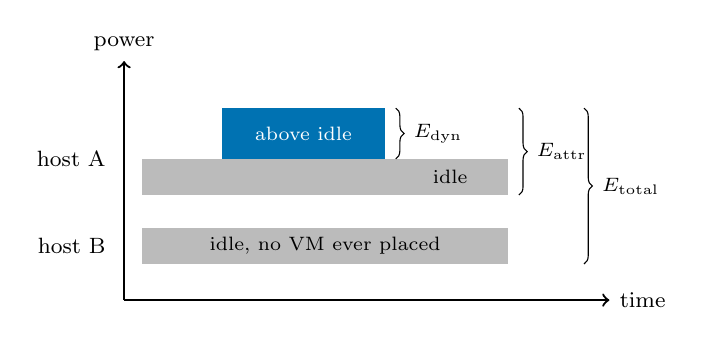
\begin{tikzpicture}[font=\small, scale=0.92]

\definecolor{idlec}{HTML}{BBBBBB}
\definecolor{dync}{HTML}{0072B2}

\draw[->, thick] (0,0) -- (6.7,0) node[right, font=\footnotesize] {time};
\draw[->, thick] (0,0) -- (0,3.3) node[above, font=\footnotesize] {power};

\node[font=\footnotesize, anchor=east] at (-0.12,1.95) {host A};
\fill[idlec] (0.25,1.45) rectangle (5.3,1.95);
\fill[dync]  (1.35,1.95) rectangle (3.6,2.65);
\node[font=\scriptsize, white] at (2.475,2.30) {above idle};
\node[font=\scriptsize] at (4.5,1.70) {idle};

\node[font=\footnotesize, anchor=east] at (-0.12,0.75) {host B};
\fill[idlec] (0.25,0.5) rectangle (5.3,1.0);
\node[font=\scriptsize] at (2.775,0.75) {idle, no VM ever placed};

\draw[decorate, decoration={brace, amplitude=3pt}]
  (3.75,2.65) -- (3.75,1.95)
  node[midway, right=3pt, font=\scriptsize] {$E_{\mathrm{dyn}}$};
\draw[decorate, decoration={brace, amplitude=3pt}]
  (5.45,2.65) -- (5.45,1.45)
  node[midway, right=3pt, font=\scriptsize] {$E_{\mathrm{attr}}$};
\draw[decorate, decoration={brace, amplitude=3pt}]
  (6.35,2.65) -- (6.35,0.5)
  node[midway, right=3pt, font=\scriptsize] {$E_{\mathrm{total}}$};

\end{tikzpicture}
\caption{The three accounting bases, shown schematically for a two-host fleet.
$E_{\mathrm{total}}$ charges every provisioned host for the whole window and is
therefore invariant to placement in a fixed fleet. $E_{\mathrm{dyn}}$ charges
only draw above idle and is unaffected by how many hosts a schedule activates.
$E_{\mathrm{attr}}$ charges the full draw of hosts that carry load and nothing
for hosts that do not, so it responds both to regional placement and to
consolidation. Host~B is provisioned in all three cases; it contributes to
$E_{\mathrm{total}}$ alone.}
\label{fig:bases}
\end{figure}
